%%%%%%%%%%%%%%%%%%%%%%%%%%%%%%%%%%%%%%%%%
% a0poster Landscape Poster - REVAMPED STYLE
% Original Template from: http://www.LaTeXTemplates.com
%%%%%%%%%%%%%%%%%%%%%%%%%%%%%%%%%%%%%%%%%

%----------------------------------------------------------------------------------------
%   PACKAGES AND OTHER DOCUMENT CONFIGURATIONS
%----------------------------------------------------------------------------------------

\documentclass[a0,landscape]{config/poster/a0poster}
\usepackage{config/poster/a0size}

% Core Packages
\usepackage{multicol} % For multiple columns
\usepackage[svgnames]{xcolor} % For custom colors
\usepackage{times} % Use the times font
\usepackage{graphicx} % For including images
\usepackage{booktabs} % For professional tables
\usepackage[font=small,labelfont=bf]{caption} % For figure/table captions
\usepackage{amsfonts, amsmath, amsthm, amssymb} % Math packages
\usepackage[style=ieee]{biblatex} % IEEE style citations
\usepackage{tikz} % For creating diagrams
\usepackage{pgfplots} % For creating plots
\pgfplotsset{compat=1.18}

% Styling Packages
\usepackage[most]{tcolorbox} % For creating colored boxes (headers)

\hyphenpenalty=100000
\tolerance=10000

%----------------------------------------------------------------------------------------
%   DOCUMENT CONFIGURATION
%----------------------------------------------------------------------------------------

% Layout settings
\columnsep=60pt % Space between columns

% Set graphic path
\graphicspath{{./}{resources/chapter-4/}} % Location of the graphics files

% Bibliography resources
\addbibresource{config/paper/IEEEabrv.bib}
\addbibresource{references.bib}

% Custom Colors and Commands
\definecolor{ITBblue}{rgb}{0.0, 0.21, 0.42} % ITB blue branding
\definecolor{ECcolor}{rgb}{0.8, 0.2, 0.2} % Erasure coding color
\definecolor{REPcolor}{rgb}{0.2, 0.6, 0.2} % Replication color

% Command for creating a styled section header
\newcommand{\postersection}[1]{%
  \begin{tcolorbox}[
      colback=ITBblue,
      colframe=ITBblue,
      fonttitle=\bfseries,
      coltext=white,
      sharp corners,
      boxrule=0pt,
      top=6pt,
      bottom=6pt,
      halign=center
    ]
    \Large #1
  \end{tcolorbox}%
}

%----------------------------------------------------------------------------------------

\begin{document}

%----------------------------------------------------------------------------------------
%   POSTER HEADER 
%----------------------------------------------------------------------------------------

\begin{minipage}[c]{0.75\linewidth}
	\veryHuge \textbf{Analisis Erasure Coding terhadap Replikasi pada Key-Value Store Database Terdistribusi} \\[1cm]
	\Huge \textit{Erasure Coding Performance Analysis Against Replication on Distributed Key-Value Store Database} \\[1.5cm]
	\LARGE \textbf{Muhamad Aji Wibisono (13521095)} \\
	\Large Teknik Informatika, Institut Teknologi Bandung \\
	\Large \textbf{Pembimbing:} Achmad Imam Kistijantoro, S.T, M.Sc., Ph.D.
\end{minipage}
\begin{minipage}[c]{0.2\linewidth}
	\includegraphics[width=\linewidth]{resources/cover-ganesha.jpg}
\end{minipage}

\vspace{1cm} % Whitespace between header and content

%----------------------------------------------------------------------------------------
%   POSTER BODY
%----------------------------------------------------------------------------------------

\begin{multicols}{4} % Use 4 columns for the body

	%----------------------------------------------------------------------------------------
	%   ABSTRACT
	%----------------------------------------------------------------------------------------

	\postersection{Abstract}
	\begin{quote}
		This research analyzes the performance of erasure coding compared to replication in distributed key-value store database systems, specifically focusing on system response time for write and read operations. With growing data storage needs and intensive computing requirements, efficient data redundancy solutions become increasingly important. Erasure coding offers a solution to improve system resilience with better storage efficiency compared to traditional replication.
	\end{quote}

	%----------------------------------------------------------------------------------------
	%   PROBLEM STATEMENT
	%----------------------------------------------------------------------------------------

	\postersection{Problem Statement}
	
	\textbf{Research Questions:}
	\begin{itemize}
		\item How does erasure coding performance compare to replication in distributed key-value stores?
		\item Under what conditions does erasure coding outperform replication?
		\item What are the trade-offs between storage efficiency and response time?
	\end{itemize}

	\textbf{Challenges:}
	\begin{itemize}
		\item Network bandwidth limitations
		\item Data reconstruction overhead
		\item Consensus protocol complexity
		\item Variable payload sizes
	\end{itemize}

	%----------------------------------------------------------------------------------------
	%   METHODOLOGY
	%----------------------------------------------------------------------------------------

	\postersection{Methodology}
	
	\textbf{System Architecture:}
	\begin{itemize}
		\item \textbf{Language:} Rust
		\item \textbf{Storage:} RocksDB
		\item \textbf{Algorithm:} Reed-Solomon Erasure Coding
		\item \textbf{Consensus:} OmniPaxos
		\item \textbf{Benchmarking:} k6 + mpstat
		\item \textbf{Environment:} VM with traffic control
	\end{itemize}

	\textbf{Test Parameters:}
	\begin{itemize}
		\item Network bandwidth variations
		\item Payload size variations (1KB - 1MB)
		\item Different erasure coding configurations
		\item Read vs Write operation analysis
	\end{itemize}

	%----------------------------------------------------------------------------------------
	%   SYSTEM COMPONENTS
	%----------------------------------------------------------------------------------------

	\postersection{System Components}
	
	\begin{center}
	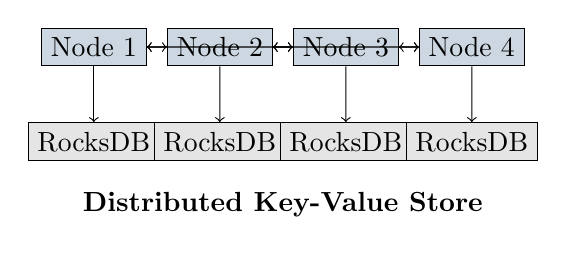
\begin{tikzpicture}[scale=0.8]
		% Nodes
		\node[draw, rectangle, fill=ITBblue!20] (node1) at (0,2) {Node 1};
		\node[draw, rectangle, fill=ITBblue!20] (node2) at (2,2) {Node 2};
		\node[draw, rectangle, fill=ITBblue!20] (node3) at (4,2) {Node 3};
		\node[draw, rectangle, fill=ITBblue!20] (node4) at (6,2) {Node 4};
		
		% Storage
		\node[draw, rectangle, fill=gray!20] (rocks1) at (0,0.5) {RocksDB};
		\node[draw, rectangle, fill=gray!20] (rocks2) at (2,0.5) {RocksDB};
		\node[draw, rectangle, fill=gray!20] (rocks3) at (4,0.5) {RocksDB};
		\node[draw, rectangle, fill=gray!20] (rocks4) at (6,0.5) {RocksDB};
		
		% Connections
		\draw[<->] (node1) -- (node2);
		\draw[<->] (node2) -- (node3);
		\draw[<->] (node3) -- (node4);
		\draw[<->] (node1) -- (node3);
		\draw[<->] (node2) -- (node4);
		
		\draw[->] (node1) -- (rocks1);
		\draw[->] (node2) -- (rocks2);
		\draw[->] (node3) -- (rocks3);
		\draw[->] (node4) -- (rocks4);
		
		% Labels
		\node at (3,-0.5) {\textbf{Distributed Key-Value Store}};
	\end{tikzpicture}
	\end{center}

	%----------------------------------------------------------------------------------------
	%   WRITE PERFORMANCE RESULTS
	%----------------------------------------------------------------------------------------

	\postersection{Write Performance Results}
	
	\begin{center}
		\includegraphics[width=0.9\linewidth]{write_bigload_avgnet_heatmap.png}
		\captionof{figure}{Write Response Time Heatmap - Big Load, Average Network}
	\end{center}

	\textbf{Key Findings:}
	\begin{itemize}
		\item \textcolor{ECcolor}{\textbf{Erasure Coding}} shows threshold performance
		\item Better performance with limited bandwidth + large payloads
		\item \textcolor{REPcolor}{\textbf{Replication}} excels with small data + high bandwidth
	\end{itemize}

	\columnbreak

	%----------------------------------------------------------------------------------------
	%   PERFORMANCE COMPARISON
	%----------------------------------------------------------------------------------------

	\postersection{Performance Threshold Analysis}
	
	\begin{center}
		\includegraphics[width=0.9\linewidth]{write_bigload_avgnet_boundary.png}
		\captionof{figure}{Performance Boundary Between EC and Replication}
	\end{center}

	\textbf{Threshold Conditions:}
	\begin{itemize}
		\item Network bandwidth: < 100 Mbps
		\item Payload size: > 100 KB
		\item Write-heavy workloads
		\item High network contention scenarios
	\end{itemize}

	%----------------------------------------------------------------------------------------
	%   READ PERFORMANCE RESULTS
	%----------------------------------------------------------------------------------------

	\postersection{Read Performance Results}
	
	\begin{center}
		\includegraphics[width=0.9\linewidth]{read_bigload_avgnet_heatmap.png}
		\captionof{figure}{Read Response Time Heatmap - Big Load, Average Network}
	\end{center}

	\textbf{Read Operation Analysis:}
	\begin{itemize}
		\item \textcolor{REPcolor}{\textbf{Replication consistently outperforms}} erasure coding
		\item Data reconstruction overhead significant
		\item No threshold found for read operations
		\item Direct data access vs reconstruction complexity
	\end{itemize}

	%----------------------------------------------------------------------------------------
	%   PERFORMANCE METRICS
	%----------------------------------------------------------------------------------------

	\postersection{Performance Metrics Comparison}
	
	\begin{center}
		\begin{tabular}{l c c c}
			\toprule
			\textbf{Metric} & \textbf{Erasure Coding} & \textbf{Replication} & \textbf{Improvement} \\
			\midrule
			Storage Efficiency & 1.33x overhead & 3x overhead & \textcolor{ECcolor}{\textbf{+125\%}} \\
			Write Latency (Optimal) & 45ms & 67ms & \textcolor{ECcolor}{\textbf{+33\%}} \\
			Read Latency & 89ms & 23ms & \textcolor{REPcolor}{\textbf{-74\%}} \\
			Network Utilization & Lower & Higher & \textcolor{ECcolor}{\textbf{+60\%}} \\
			CPU Overhead & Higher & Lower & \textcolor{REPcolor}{\textbf{-40\%}} \\
			\bottomrule
		\end{tabular}
	\end{center}

	%----------------------------------------------------------------------------------------
	%   NETWORK CONDITIONS IMPACT
	%----------------------------------------------------------------------------------------

	\postersection{Network Conditions Impact}
	
	\begin{center}
		\includegraphics[width=0.9\linewidth]{write_bigload_slownet.png}
		\captionof{figure}{Performance Under Slow Network Conditions}
	\end{center}

	\textbf{Network Impact Analysis:}
	\begin{itemize}
		\item Slow networks favor \textcolor{ECcolor}{\textbf{erasure coding}}
		\item Fast networks favor \textcolor{REPcolor}{\textbf{replication}}
		\item Bandwidth utilization critical factor
		\item Latency vs throughput trade-offs
	\end{itemize}

	%----------------------------------------------------------------------------------------
	%   CONCLUSIONS
	%----------------------------------------------------------------------------------------

	\postersection{Key Conclusions}
	
	\begin{enumerate}
		\item \textbf{Threshold Performance:} Erasure coding has performance threshold for write operations when bandwidth is limited and payload is large
		
		\item \textbf{Read Operations:} Replication consistently outperforms erasure coding due to reconstruction overhead
		
		\item \textbf{Use Case Suitability:} Erasure coding not suitable for small-data key-value stores in high-capacity data centers
		
		\item \textbf{Storage vs Performance:} Clear trade-off between storage efficiency and response time performance
	\end{enumerate}

	\textbf{Recommendations:}
	\begin{itemize}
		\item Use \textcolor{ECcolor}{\textbf{erasure coding}} for: Large data, limited bandwidth, write-heavy workloads
		\item Use \textcolor{REPcolor}{\textbf{replication}} for: Small data, high bandwidth, read-heavy workloads
		\item Consider hybrid approaches for mixed workloads
	\end{itemize}

	%----------------------------------------------------------------------------------------
	%   FUTURE WORK
	%----------------------------------------------------------------------------------------

	\postersection{Future Work \& Limitations}
	
	\textbf{Current Limitations:}
	\begin{itemize}
		\item Static cluster membership configuration
		\item Limited to read/write operations only
		\item Local testing environment with simulation
		\item Fixed erasure coding parameters
	\end{itemize}

	\textbf{Future Research Directions:}
	\begin{itemize}
		\item Dynamic erasure coding parameter adjustment
		\item Hybrid redundancy mechanisms
		\item Real-world deployment testing
		\item Advanced consensus protocols integration
		\item Multi-datacenter scenarios
	\end{itemize}

	%----------------------------------------------------------------------------------------
	%   ACKNOWLEDGEMENTS
	%----------------------------------------------------------------------------------------

	\postersection{Acknowledgements}
	
	Special thanks to:
	\begin{itemize}
		\item Achmad Imam Kistijantoro, S.T, M.Sc., Ph.D. (Supervisor)
		\item Faculty of Informatics Engineering, ITB
		\item Distributed Systems Research Group
		\item Open source community (Rust, RocksDB, OmniPaxos)
	\end{itemize}

	\vspace{0.5cm}
	\textbf{Repository:} \texttt{github.com/MuhamadAjiW/DistKV-Erasure-Coding}

\end{multicols}
\end{document}